% Created 2013-01-28 Mon 22:41
\documentclass[11pt]{article}
\usepackage{graphicx}
\usepackage{geometry}
\usepackage{amsmath}
\usepackage[pdftex]{hyperref}
\usepackage[font=small,labelfont=bf]{caption}
\geometry{a4paper, textwidth=6.5in, textheight=10in, marginparsep=7pt, marginparwidth=.6in}

\title{Data Mining 2013: Project Report}
\author{vcarbune@ethz.ch\\ mgrecu@ethz.ch}
\date{\today}

\begin{document}
\maketitle

\section{Approximate retrieval - Locality Sensitive Hashing}
\begin{enumerate}
\item How was your choice of rows and bands motivated? How did you search for the
best parameters? \\

\textbf{Answer}: \\
Initially, we considered to use the maximum available number of
hash functions. We tried different combinations where the product 
between rows and bands is close to the maximum (120).

The scores obtained have indicated that a lower number of bands yield
better results. Therefore we continued with testing configurations where 
the number of bands was lower than the number of rows. 
We also looked at cases where the product between the number of bands and
the number of rows is much lower than the maximum. 
There seemed to be a lot of local maxima and there wasn't any clear pattern 
which combinations yield the best scores. We got the best scores by using
between 3 and 7 bands and between 10 and 20 rows.
Surprisingly, we got the best score when we only used 3 bands and 12 rows.


\begin{figure}[h!b]
\centering
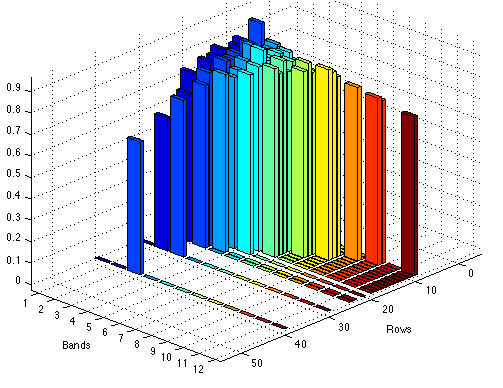
\includegraphics[width=0.7\textwidth]{lsh.png}
\caption{F1 scores for different parameter combinations}
\label{fig:lsh_chart}
\end{figure}


\item Conceptually, what would you have to change if you were asked to design an image
  retrieval system that you can query for similar images given a large image
  dataset? \\

\textbf{Answer}: First, we would have extracted patches of 8 x 8 pixels
(standard patch size used in Computer Vision) from all the images we
have. Instead of the k-shingles used for documents, we would have used patches
similarly to describe images in the given collection. The next step
would have been to cluster these and identified representative features
for the image collection. Further, we would have applied LSH for an
incoming image by decomposing it into its representative patches and
used the same technique as we did for the document.

\end{enumerate}

\section{Large-scale Supervised Learning}

\begin{enumerate}
\item Which algorithms did you consider? Which one did you choose for the
  final submission and why? \\
  
\textbf{Answer}: We considered multiple algorithms. We started with the
ones presented in the course and continued the implementation using
algorithms presented in \cite{Sculley09}.

We have started with the simple version of the online SVM learning
algorithm, presented in the Data Mining course. The training samples
were initially given sequentially to test the functionality itself, and
after that randomly.

The second step was to implement the improved version, Pegasos SVM. We
had tested our algorithm with different values for lambda and for the number 
of training epochs. 
Besides the documentation available in the course, we also used
a set of ideas presented in a blog post\footnote{
http://bickson.blogspot.ch/2012/04/more-on-large-scale-svm.html}.

We achieved good performances with Pegasos SVM, but wanted to further
explore the field and try out several other approaches. The next
immediate approach that seemed to yield good results was training
minibatches, instead of one sample at a time. This approach indeed
obtained constantly good results (without strong variations from one
submission to another).

Two aspects are relevant to consider and evaluate when talking about
Pegasos in conjunction with minibatches: how we built the minibatch and
how we updated the weights. Regarding the subset construction, we have
tried two different approaches:
\begin{itemize}
\item{Sampling uniformly at random from the initial data set in order
to obtain a minibatch of a fixed size.}
\item{Construct minibatches such that the union of all minibatch sets 
is equal to the initial data set, building a complete and disjoint coverage.}
\end{itemize}

Among these, the first one yielded slightly better results. Enforcing a
complete and disjoint coverage of the initial set isn't a \emph{natural}
setting of the problem, while bootstrapping, resampling with replacement
from the initial data set, efficiently resembles the initial problems
and optimally updates the weights.

The weight update is done after an intermediate sum of the minibatch is
computed, instead of updating it each time a new sample is encountered.

Besides these algorithms, we have also implemented ROMMA, Balanced
Pegasos (updating weights is always done by considering a positive and a
negative example). Both of these are extensively discussed in \cite{Sculley09}, 
and we followed the suggestions from there, but performances weren't improved.

For the final submission we sticked with the basic Pegasos algorithm, with a few twists.
First of all, we traverse the data set on one machine multiple times (epochs), 
and before each traversal we shuffle the list of samples. 
We also introduced a bias factor for false positives. Considering that the cost of 
misclassification of a false positive is four times higher than that of a false negative, 
we decided that each time we encounter such a value, we give a higher weight 
for the movement towards the data point that was misclassified as positive.

% Not true: [However, on average, Pegasos with Minibatches yielded better results.]

\item How did you select the parameters for your model? Which are the
  most important parameters of your model? \\
  
\textbf{Answer}:  The parameters to be considered for discussion are the following:
\begin{itemize}
\item{\textbf{Number of machines:}} We tried different values, but we got the best scores 
when we used either around 100 machines or around 20 machines.
\item{\textbf{Lambda:}} We tried several possibilities, varying the
magnitude order: $10^{-6}, 10^{-5}, 10^{-4}$, etc. In the end, the best
outcome was obtained using values around $10^{-5}$.
\item{\textbf{Epochs:}} Considering the execution time of the program, we only tried 
varying the number of epochs from 1 to 5. We got the best scores when we used 2 or 3 
epochs.
\item{\textbf{Bias factor:}} Considering the cost ratio of 1:4 between false positives 
and false negatives, we tried using a bias factor around this ratio, between 1.0 and 5.0.
The best scores were obtained with a bias factor of around 2.0.

Each algorithm introduced its own set of parameters, on top or instead
of the ones mentioned above. For example mininbatches, for which we
obtained on average very good scores (but not the best), we also tuned
the \textbf{minibatch size} and \textbf{epochs}. Depending on the
construction of the minibatch, usually we thought about keeping the
product $ size * epochs $ constantly equal to the total number of
samples (as this would increase the probability that the minibatches
obtained through resampling with replacement would cover the complete
initial size).

\end{itemize}

\end{enumerate}

\section{Recommender Systems}

\begin{enumerate}
\item Which algorithm did you implement? What was your motivation? \\ \\
\textbf{Answer}:

TODO(vcarbune): LinUCB, LinUCBHybrid.


Considering the fact that there was a limit on the execution time, we had to 
optimize all the matrix operations. Basically, we tried to use the main memory to store
some matrices for each article, so that we don't have to recompute them every time we
have to perform an action. For example, for an article \emph{a} we store the matrix
$A_a ^ {-1}$ in memory. And we only update the matrices for one article when we get 
feedback from the action. Due to this, we could do all the steps in the algorithm for
the entire dataset and still fit into the time limit. 

We also used the fact that the performance of an article degrades over time. 
In the formula for the score $p_{t,a}$ of an article \emph{a} at time \emph{t}, we also
subtract a value that depends on the age of the article: 
$p_{t,a} \gets p_{t,a} - c \cdot f(age_a)$, 
where $age_a$ - the age of \emph{a} in seconds.

\item How did you select the parameters for your model? \\ \\
\textbf{Answer}:

The parameters that we could vary in both LinUCB and LinUCB-Hybrid were: 
the constant $\alpha$, the function \emph{f} and the constant \emph{c}.

For $\alpha$, the theoretical results suggest a value higher than 1. To get a confidence
level of $99\%$, $\alpha$ should be around 4. 
But we tried with values of all magnitudes, and we got the best results for values around
0.1 - 0.2.

To include the age of the article in the score formula, we tried two functions: 
\begin{itemize}
    \item $f(age_a) = age_a$.
    \item $f(age_a) = log_{10}(age_a)$.
\end{itemize}

The second option gave better results. The constant \emph{c} in the formula for $p_{t,a}$
was chosen so that it makes the value of \emph{f} about one order of magnitude less than
the value of $p_{t,a}$. More specifically, it was chosen to be around 0.001 - 0.005.

\item Does the performance measured in CTR increase monotonically during the
execution of your algorithm? Why? \\ \\
\textbf{Answer}: No, the performance is not increasing monotonically.
It happens that, as more and more samples are included in our
computations, not all of them immediately improve the results.
Consider a sample that is not a click-through ad, but it tells us a lot
about the preferences not relevant for CTR. We do want to take it into
account, even if its immediate impact is to lower a bit the score.

Without decreasing it the CTR might drop even more later, so it is
important for us to take in consideration as much of the data as
possible.

\end{enumerate}


\begin{thebibliography}{100}

\bibitem{Sculley09} Sculley, D., \emph{Large scale learning to rank.} 
NIPS Workshop on Advances in Ranking. 2009.

\end{thebibliography}

\end{document}
